\documentclass[11pt,a4paper]{article}
\usepackage[utf8]{inputenc}
\usepackage{amsmath}
\usepackage{amsfonts}
\usepackage{amssymb}
\usepackage{float}
\usepackage{fullpage}

\usepackage{graphicx}
\graphicspath{{./images/}}

\begin{document}

\begin{titlepage}
\begin{center}

% Upper part of the page. The '~' is needed because \\
% only works if a paragraph has started.


\textsc{\LARGE Delft University of Technology}\\[1.5cm]

\textsc{\Large IN4010 Practical Assignment 2}\\[0.5cm]

% Title
%\HRule \\[0.4cm]
{ \huge \bfseries Agent assessment and improvement \\[0.4cm] }

%\HRule \\[1.5cm]

% Author and supervisor
\noindent
\begin{minipage}{0.4\textwidth}
\begin{flushleft} \large
\emph{Group 11:}\\
Hidde \textsc{Coehoorn}\\
Ralf \textsc{Nieuwenhuizen}\\
Jan-Willem \textsc{van Velzen}
\end{flushleft}
\end{minipage}%
\begin{minipage}{0.4\textwidth}
\begin{flushright} \large
\emph{Supervisor:} \\
Reyhan \textsc{Aydogan}
\end{flushright}
\end{minipage}

\vfill

% Bottom of the page
{\large \today}

\end{center}
\end{titlepage}

\newpage
\section{Test Description}

After finishing the first version of our own negotiation agent, we were provided with the negotiation agents of other groups and their domains. We decided to do a comprehensive set of tests in the genius Tournament environment. 10 Tournaments were ran, for every opponent-profile combination of three parties per tournament, resulting in 2\textsuperscript{3} = 8 sessions per tournament. All opponents were tested in their own domain, with the following exceptions:

\begin{itemize}
	\item Opponent 9 was not tested, because we were unable to get the agent running. 
	\item Opponent 10 was tested on the domain of Opponent 12, because the domain of Opponent 10 was missing.
\end{itemize}

We were unable to determine which domain, provided by Opponent 2, was the cooperative, moderate and competitive domain, so we made the alphabetical assumption of \textit{Dinner}, \textit{Sporthal} and \textit{Politics} respectively. \\

We also note that sessions were only counted when an agreement was reached as shown in Figure \ref{fig:18_agreements} and \ref{fig:180_agreements}. This resulted in less data for Opponent 2, 6, 7 and 10, specifically for the variables: Distance to Pareto, Distance to Nash, Social Welfare, and the Utilities.

\begin{figure}[!htb]
	\minipage{0.49\textwidth}
	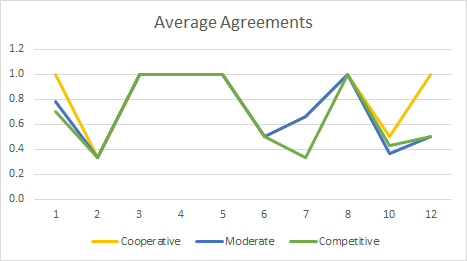
\includegraphics[width=\linewidth]{pre/18_agreements}
	\caption{18 Rounds per Opponent}
	\label{fig:18_agreements}
	\endminipage\hfill
	\minipage{0.49\textwidth}
	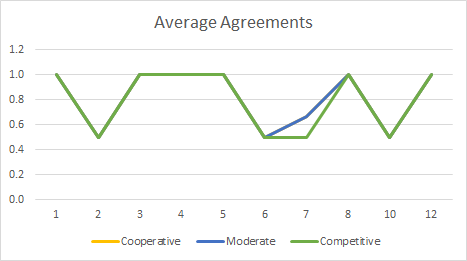
\includegraphics[width=\linewidth]{pre/180_agreements}
	\caption{180 Rounds per Opponent}
	\label{fig:180_agreements}
	\endminipage\hfill
\end{figure}

These tests were done twice, for both 18 and 180 maximal tournament rounds.
All results were then averaged over all sessions and domain types, ignoring the sessions with the following agent composition: n/n/n and 11/11/11. All these combined test resulted in a dataset of a whopping (60 $\cdot$ 30 $\cdot$ 2 =) 3600 sessions.

\newpage
\section{Test results}

After performing the described tests we ended up with quite a lot of data. The various test results are summarized in figures, some of which are included further on in this chapter to illustrate interesting and valuable observations.

\subsection{Agreements}

Looking at the Average test agreements in Figure \ref{fig:18_agreements} and \ref{fig:180_agreements}, we see that with a tighter deadline, we achieve less agreements compared to the scenario with a 180-round cap.

\begin{figure}[H]
	\minipage{0.49\textwidth}
	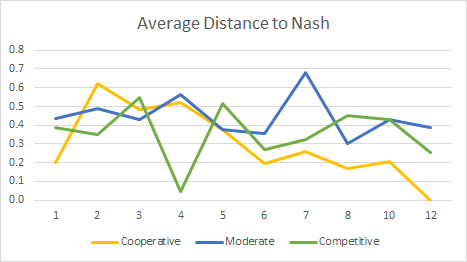
\includegraphics[width=\linewidth]{pre/18_distance_nash}
	\caption{18 Rounds per Opponent}
	\label{fig:18_distance_nash}
	\endminipage\hfill
	\minipage{0.49\textwidth}
	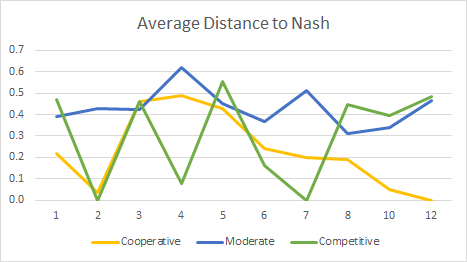
\includegraphics[width=\linewidth]{pre/180_distance_nash}
	\caption{180 Rounds per Opponent}
	\label{fig:180_distance_nash}
	\endminipage\hfill
\end{figure}

\subsection{Distances to Nash and Pareto}

Figures \ref{fig:18_distance_nash} and \ref{fig:180_distance_nash} show the average distance to Nash for each set of tournaments. We see that on the longer negotiations, bids with a lower distance to Nash are found and used. This results in lower distances to Nash. The same can be observed from the average distance to Pareto in Figure \ref{fig:18_distance_pareto} and \ref{fig:180_distance_pareto}.

\begin{figure}[H]
	\minipage{0.49\textwidth}
	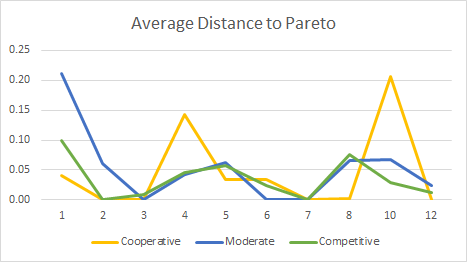
\includegraphics[width=\linewidth]{pre/18_distance_pareto}
	\caption{18 Rounds per Opponent}
	\label{fig:18_distance_pareto}
	\endminipage\hfill
	\minipage{0.49\textwidth}
	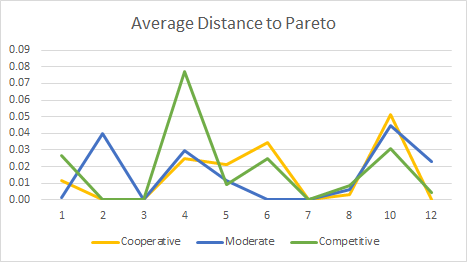
\includegraphics[width=\linewidth]{pre/180_distance_pareto}
	\caption{180 Rounds per Opponent}
	\label{fig:180_distance_pareto}
	\endminipage\hfill
\end{figure}

\subsection{Number of Rounds}

The number of rounds it takes to reach an agreement (Figure \ref{fig:18_rounds} and \ref{fig:180_rounds}) is relatively the same for both 18- and 180-capped sessions. It can also be observed that the opponents that we reach a lower amount of agreements with, generally take more rounds to that agreement.\\

\begin{figure}[H]
	\minipage{0.49\textwidth}
	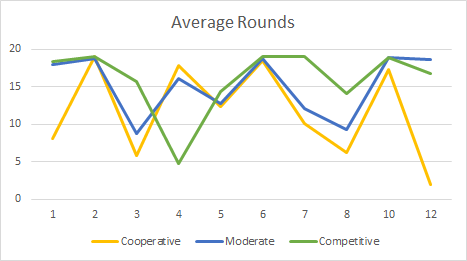
\includegraphics[width=\linewidth]{pre/18_rounds}
	\caption{18 Rounds per Opponent}
	\label{fig:18_rounds}
	\endminipage\hfill
	\minipage{0.49\textwidth}
	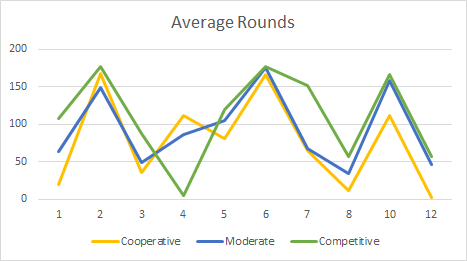
\includegraphics[width=\linewidth]{pre/180_rounds}
	\caption{180 Rounds per Opponent}
	\label{fig:180_rounds}
	\endminipage\hfill
\end{figure}

\subsection{Social Welfare}

Despite the bigger distances to Nash and Pareto, Figure \ref{fig:18_social_welfare} and \ref{fig:180_social_welfare} show that the average Social Welfare for both short and long negotiations are practically identical. \\

\begin{figure}[H]
	\minipage{0.49\textwidth}
	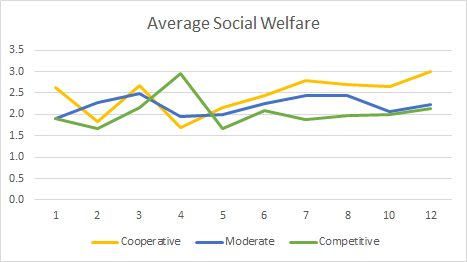
\includegraphics[width=\linewidth]{pre/18_social_welfare}
	\caption{18 Rounds per Opponent}
	\label{fig:18_social_welfare}
	\endminipage\hfill
	\minipage{0.49\textwidth}
	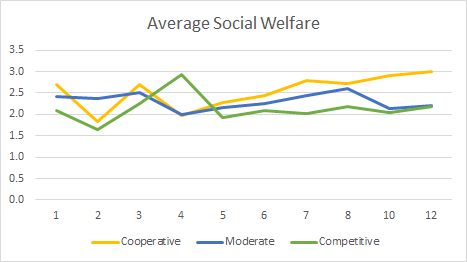
\includegraphics[width=\linewidth]{pre/180_social_welfare}
	\caption{180 Rounds per Opponent}
	\label{fig:180_social_welfare}
	\endminipage\hfill
\end{figure}

\subsection{Cooperative utilities}

Finally we take a look at the achieved utilities. Starting with cooperative in Figure \ref{fig:18_utils_domain_cooperative} and \ref{fig:180_utils_domain_cooperative}, we perform less in the long negotiation compared to the short negotiation. On average we perform equal to our opponents in the short negotiations, where we are clearly outperformed in the long run.\\

\begin{figure}[H]
	\minipage{0.49\textwidth}
	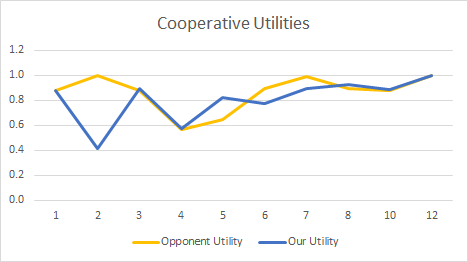
\includegraphics[width=\linewidth]{pre/18_utils_domain_cooperative}
	\caption{18 Rounds per Opponent}
	\label{fig:18_utils_domain_cooperative}
	\endminipage\hfill
	\minipage{0.49\textwidth}
	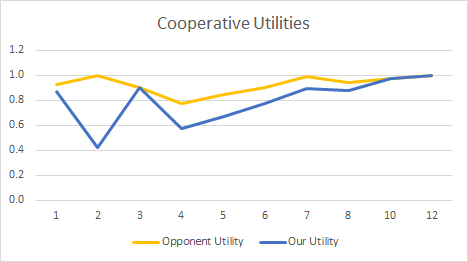
\includegraphics[width=\linewidth]{pre/180_utils_domain_cooperative}
	\caption{180 Rounds per Opponent}
	\label{fig:180_utils_domain_cooperative}
	\endminipage\hfill
\end{figure}

\subsection{Moderate utilities}

Secondly the utilities from the moderate domain, shown in Figure \ref{fig:18_utils_domain_moderate} and \ref{fig:180_utils_domain_moderate}. Again, these are mostly equal, with the exception of Opponent 5 outperforming us and Opponent 12 performing less (in the long negotiations). 

\begin{figure}[H]
	\minipage{0.49\textwidth}
	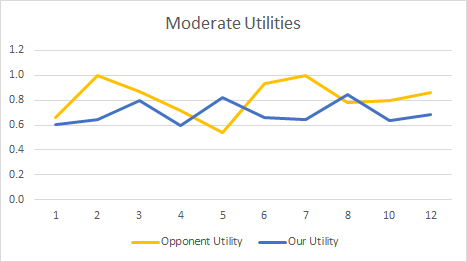
\includegraphics[width=\linewidth]{pre/18_utils_domain_moderate}
	\caption{18 Rounds per Opponent}
	\label{fig:18_utils_domain_moderate}
	\endminipage\hfill
	\minipage{0.49\textwidth}
	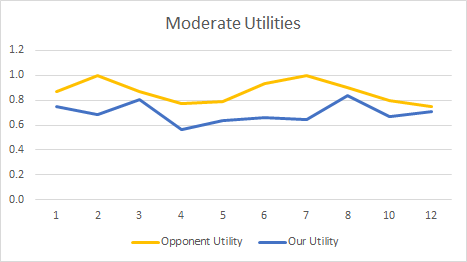
\includegraphics[width=\linewidth]{pre/180_utils_domain_moderate}
	\caption{180 Rounds per Opponent}
	\label{fig:180_utils_domain_moderate}
	\endminipage\hfill
\end{figure}

\subsection{Competitive utilities}

Without trying to sound too repetitive, looking at the competitive utilities in  Figure \ref{fig:18_utils_domain_competitive} and \ref{fig:180_utils_domain_competitive}, we see again that opponent 5 and 12 seem to have the same behavior when comparing the short and long negotiations, with our own performance being less in the long term.

\begin{figure}[H]
	\minipage{0.49\textwidth}
	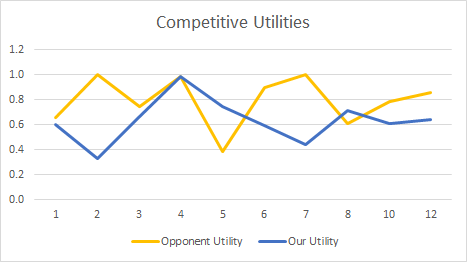
\includegraphics[width=\linewidth]{pre/18_utils_domain_competitive}
	\caption{18 Rounds per Opponent}
	\label{fig:18_utils_domain_competitive}
	\endminipage\hfill
	\minipage{0.49\textwidth}
	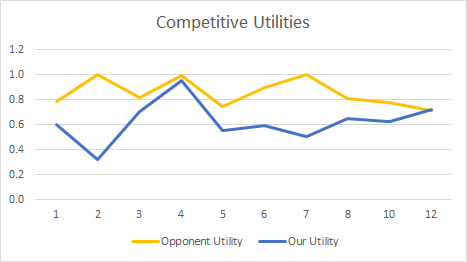
\includegraphics[width=\linewidth]{pre/180_utils_domain_competitive}
	\caption{180 Rounds per Opponent}
	\label{fig:180_utils_domain_competitive}
	\endminipage\hfill
\end{figure}

\newpage
\section{Adaptations}
Considering the test results, certain improvements should be made to the agent, to improve the results against other agents.

\subsection{Parameter changes}
Based on the first version of the agent, there are several adaptations that can be made. Simple changes are the altering of parameters, mostly numerical values, that determine when and how fast actions are taken by the agent. Examples are in the list below.

\begin{itemize}
\item The ReservationValue starts decreasing automatically after a certain amount of time. In the first version this happened at $85\%$ of time. This can be increased to be less sensitive to the opponent's preferences. It can also be decreased to be more sensitive.
\item If the previous bid has been accepted by enough other agents, the ReservationValue is also decreased. This currently happens by a multiplication by $0.8$. Increasing this value towards $1$ will make the agent less sensitive to the opponent's preferences. Decreasing it towards $0$ will make it more tolerant.
\item When there is no time to create a trusted opponent model, the GiveIn tactic is used. This creates a more tolerant offer each round. The amount of tolerance added each round can be adjusted.
\item \emph{numberOfRoundsForOpponentModel}. This parameter determines the border between a short negotiation and a long negotiation. We can play around with it to see what gives the best opponent model.
\end{itemize}


\subsection{Strategy changes}
Apart from the parameter changes, the bidding and accepting strategy of the agent can also be modified. 
 
\begin{itemize}
\item Introduce an ``AcceptanceValue'' that represents a value above which the agent will always accept. Currently this is partly represented by the ReservationValue, but that is not what the ReservationValue is meant for.
\item Do not bluntly accept after $95\%$ of the time has passed when the GIVEIN strategy is used, but instead try to make a reasonable offer around the reservation value.
\item NOSTALGIAN is always the best possible bid - maybe make it the best bid from the opponent?
\item Make smart determination when the opponent model is good?
\end{itemize}

\section{Adaptation results}

\newpage
\section{Conclusions and recommendations}
After all the tests we have performed, we can conclude that our agent was a bit to tolerant at first, and after tweaking some of the parameters to make it less tolerant, it performed better for itself, and even improved the social wellfare a bit.
\\\\
For future improvements, the changes mentioned in section \ref{sec:strategy-changes} could still be implemented. When it turns out that this agent is good enough to make it to the ANAC, we will certainly do that.

\end{document}